\documentclass[12pt]{report}
\usepackage[a4paper]{geometry}
\usepackage[myheadings]{fullpage}
\usepackage{fancyhdr}
\usepackage{lastpage}
\usepackage[T1]{fontenc}
\usepackage[font=small, labelfont=bf]{caption}
\usepackage{fourier}
\usepackage[protrusion=true, expansion=true]{microtype}
\usepackage[english]{babel}
\usepackage{sectsty}
\usepackage{url, lipsum}
\usepackage{siunitx, graphicx, array, multirow, colortbl, wrapfig, subcaption, setspace, booktabs}
\usepackage[table]{xcolor}
\usepackage[export]{adjustbox}
\usepackage{comment}

\newcommand{\HRule}[1]{\rule{\linewidth}{#1}}
\onehalfspacing
\setcounter{tocdepth}{5}
\setcounter{secnumdepth}{5}

% header and footer
\pagestyle{fancy}
\fancyhf{}
\setlength\headheight{15pt}
\fancyhead[L]{MSU Chatroom Project Report}
\fancyhead[R]{Erem Ekici, Sammy Samkough}
\fancyfoot[R]{Page \thepage\ of \pageref{LastPage}}

% title page
\begin{document}

\title{ \normalsize \textsc{CSIT340 - Computer Networks}
		\\ [0.5cm] \HRule{0.5pt} \\
		\LARGE \textbf{\uppercase{MSU Chatroom}}
		\HRule{0.5pt} \\ [0.5cm]
		\normalsize \today \vspace*{5\baselineskip}}

\date{}

\author{
        Professor Dawei Li \\
		Montclair State University \\
		Erem Ekici, Sammy Samkough }

\maketitle
\tableofcontents
\newpage

% section title format
\sectionfont{\scshape}

% body
\section{Introduction}
For this project, we were assigned to design and implement a chat room server and client using UDP socket programming. To start things off, a chat room is defined as an application where multiple clients (i.e. humans) could send messages back and forth to one another. The server's role in this is to retrieve the messages and broadcast it to all clients, while the client's role is to simply receive and send messages. \\

\noindent
We're using UDP socket programming rather than TCP socket programming in this project. There are significant differences between the two protocols. UDP is simpler than TCP, and easier to implement. It sends messages to a UDP socket by encapsulating a UDP datagram, which is then encapsulated into an IP datagram and then sent to said UDP socket destination. The issue with this protocol is that it's unreliable - there's no guarantee that the message will be sent to the UDP socket, as well as the order of datagrams be accurate. The key thing in UDP is that there is no connection between the client and the server which is why we call this a connectionless protocol. TCP on the other hand is the complete opposite, it is a connected protocol because it creates a connection between the client and server. TCP has reliability to it because when the TCP client sends a message to the server, it needs to hear an acknowledgement back from the server. If the acknowledgement isn't received, TCP doesn't send the message. \\

\noindent
We were allowed to either build our chat room application in Python or Java. We chose to go with Python due to its elegant and simple syntax, as well as it being much lighter than a Java application would. Python also doesn't require as many imports and lines as Java does, which makes it much more easier, comprehensible, and simple to implement. \\

\noindent
The main challenges we had was not the design - that was easy. Thinking of what was needed and required was relatively simple. What our main challenges were was how to syntactically write and implement it. We didn't know exactly how to write it. Although we had projects which touched upon what was supposed to be done for the chat room, there were still some things left behind that weren't brought up. For example, creating and maintaining threads was a challenge of our's that was intimidating at first. Another challenge was ensuring that we broadcast to all clients and that it reaches them. Sending the message out was the easy part, the annoying part to verify is to ensure that all clients received the message asynchronously through threads. This is just one example. \\

\noindent
These challenges were addressed by on-going tests that were done to verify our designs. We also referred to resources to give us hints and how to build some functions. We knew how to design it within pseudocode, but implementing it became a problem. These challenges were also met by constantly thinking of the most efficient way to do something, as well as not overthinking the implementation. It's relatively simple and easy to understand, so once we had that down implementing it became a lot easier.

\section{Design and Implementation}
The server includes a broadcast function and a while loop designed to run infinitely. The while loop will continuously wait to receive messages and immediately broadcast them out to each recorded client. Within the while loop is a condition such that if the message is only "join" it will automatically add the client to the list of addresses to be broadcasted to. If the client is already listed, it will be noted and not duplicated. The other potential command is "{quit}" which will remove a client from the address list. Since we use an infinite loop to receive messages, the server will never miss a message, and instantly changes the address list if needed. The server will also send the received message back to the client that sent it, in addition to each other client, in order to let them know what they sent and that their message had been received. \\

\noindent
The client has a receive and a send function. Acknowledging that the clients had to be able to simultaneously receive and send messages at any time, we chose to implement intentionally infinite loops and multi-threading. The receive function is an infinite loop that will always be prepared to receive and print a message, and is threaded so it can run at the same time as any other threaded function that we could add to the client. The send function is also an infinite loop that will keep asking the user to type a message in, and is threaded so it can run at the same time as any other threaded function we could add. When the client starts, it automatically sends the message "join" to the server. When the server receives the message "join" it adds the client to the list of addresses to broadcast received messages to. \\

\noindent
The server has an array called clients that will list each address the server will broadcast messages to. The servers while loop includes several command checks such as "join" and "{quit}". After checking the message, if it is "join" it will loop through the clients list to see if the address is already there, if not it will add it to this list, and broadcast that a new client has joined the chat room. Otherwise, it will simply state it is a duplicate client and do nothing. If the message is "{quit}" it will remove the client from the clients list and broadcast that this client has left the chat room. If the message is neither command, it will broadcast the message to each client in the clients list. \\

\noindent
The client has two threaded infinite loops, one called receive, and the other send. Neither command requires a parameter. Receive will try to receive a message from the server over and over, whenever it successfully receives a message, it will print it out for the client. Send will try to receive input from the client over and over, whenever it receives input it will send the message to the server, and then check if the message is "{quit}". If the message is quit, send sets itself to false and stops running.

\section{Testing}
There were several requirements that needed to be met for this project. Some were obvious while some others weren't so obvious. The main requirements for the server was to ensure that it would connect with clients, receive messages from clients, broadcast messages to all clients, and remove a client when it wanted to exit the application. The main requirements for the client was to ensure that it would connect with the server, receive messages (mainly broadcast) from the server, send messages to the server, and exit the application. In order to implement these requirements, heavy testing was done to always check whether something was sent, received, added, deleted, and we would always print to the console to see the results. \\

\noindent
For the server, there were some requirements that were hard to tell whether they happened correctly or not. For example, when designing the broadcast function it's simple - whenever a client wants to send a message, loop a list of clients and send it to them. We would always do that correctly, but the issue was that some clients weren't receiving messages, or it would be delayed. This made us confused and would sometimes have us think it would be the server's problem, but in reality it was how the client was handling the receiving. \\

\noindent
Another example is when a client joins, we wanted to ensure that there were no duplicates. We did this by first, randomizing the port number the client uses. Although this works most of the time, there still might be cases where clients have the same port number. So what we did was when the client joins, we immediately check if it's a duplicate by looping through all clients and seeing if the client that just joined is equal to a client on the list. If it is, don't add it to list. If it isn't, add to list. Figure 1 shows the implementation. \\

\begin{center}
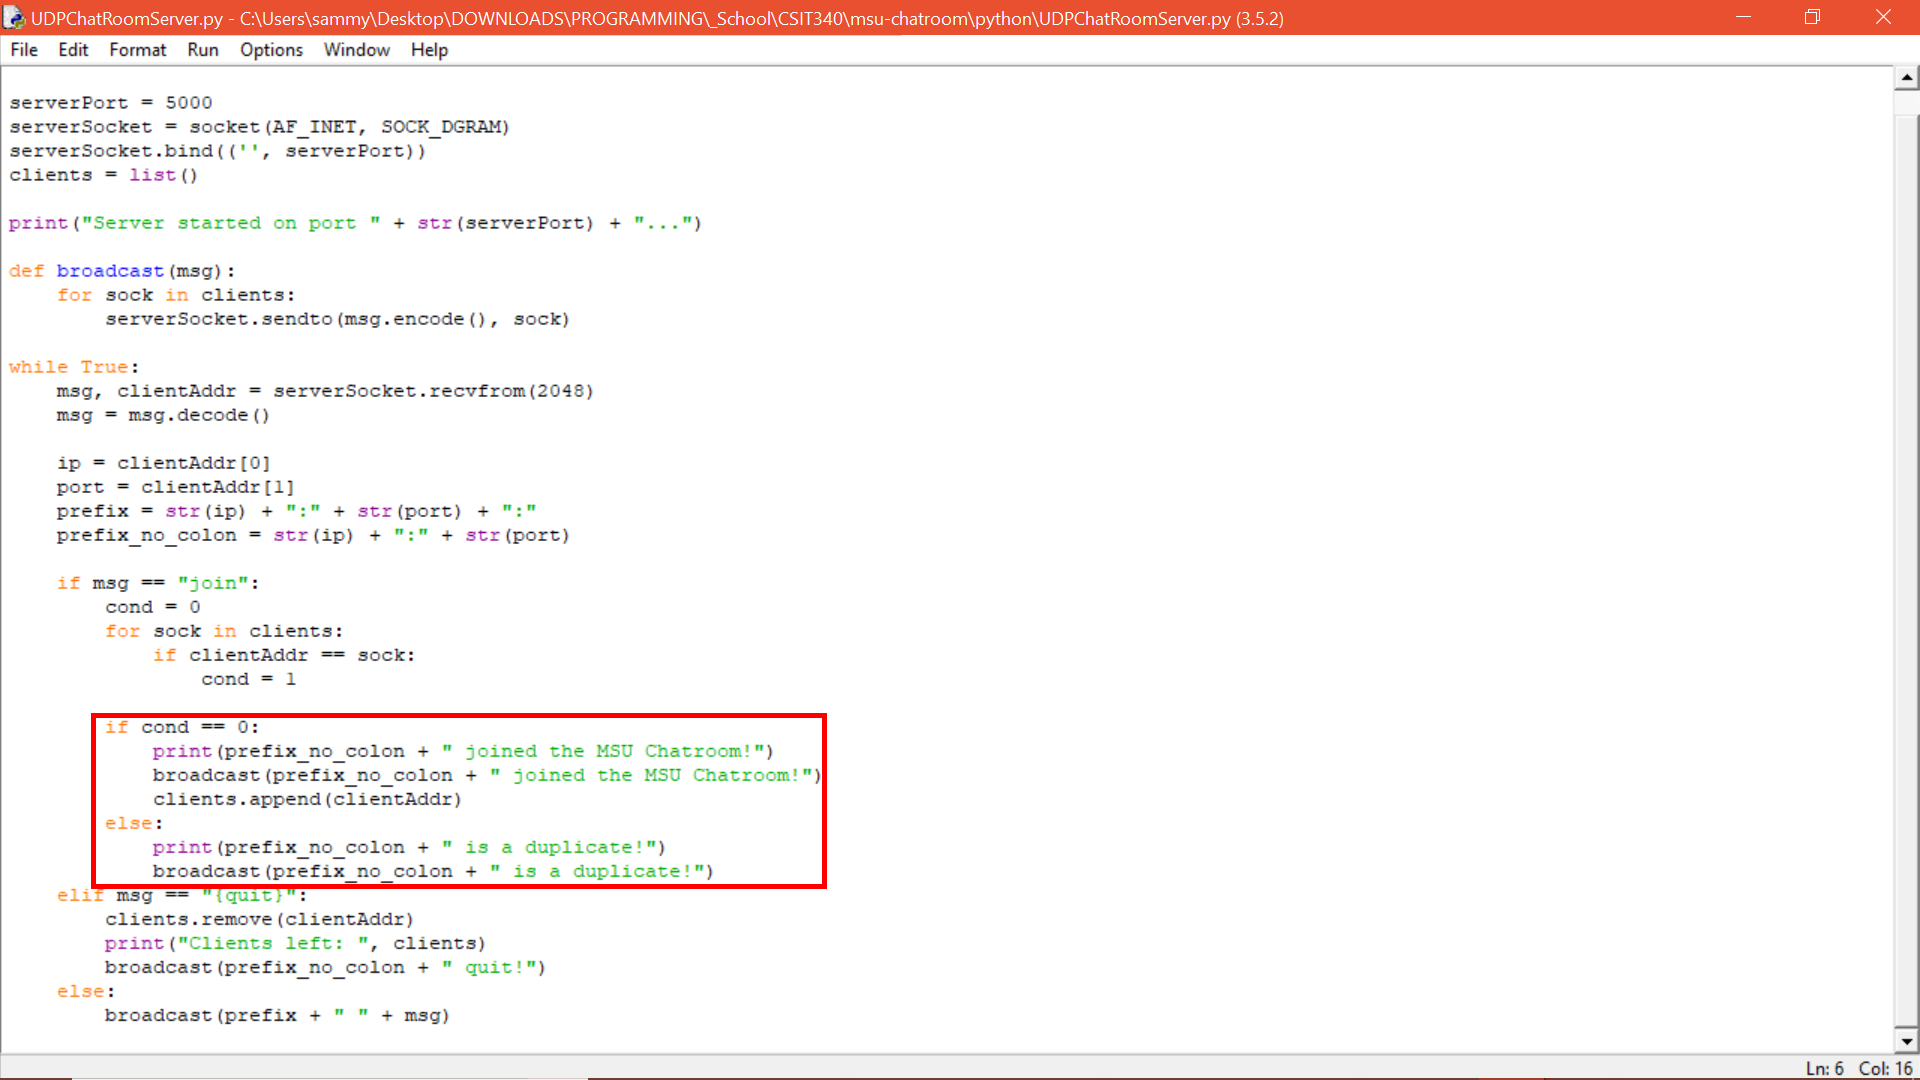
\includegraphics[scale=.25]{test-case-duplicates.png}\\
\captionof{figure}{Test Case - Duplicate}
\end{center} \\

\noindent
Our final example for a server requirement that needed a test case was when a client wanted to exit the application, we had to make sure that we delete the client from the list and then broadcast a message to all clients saying that the client left. We didn't want the client to receive the message that it's quitting because it should quit right away, it doesn't need to see that. What we did to make sure the client deletion was working is we would print the list before we would execute it, and after as well to see if the client is still on the list. Figure 2 shows the implementation. \\

\begin{center}
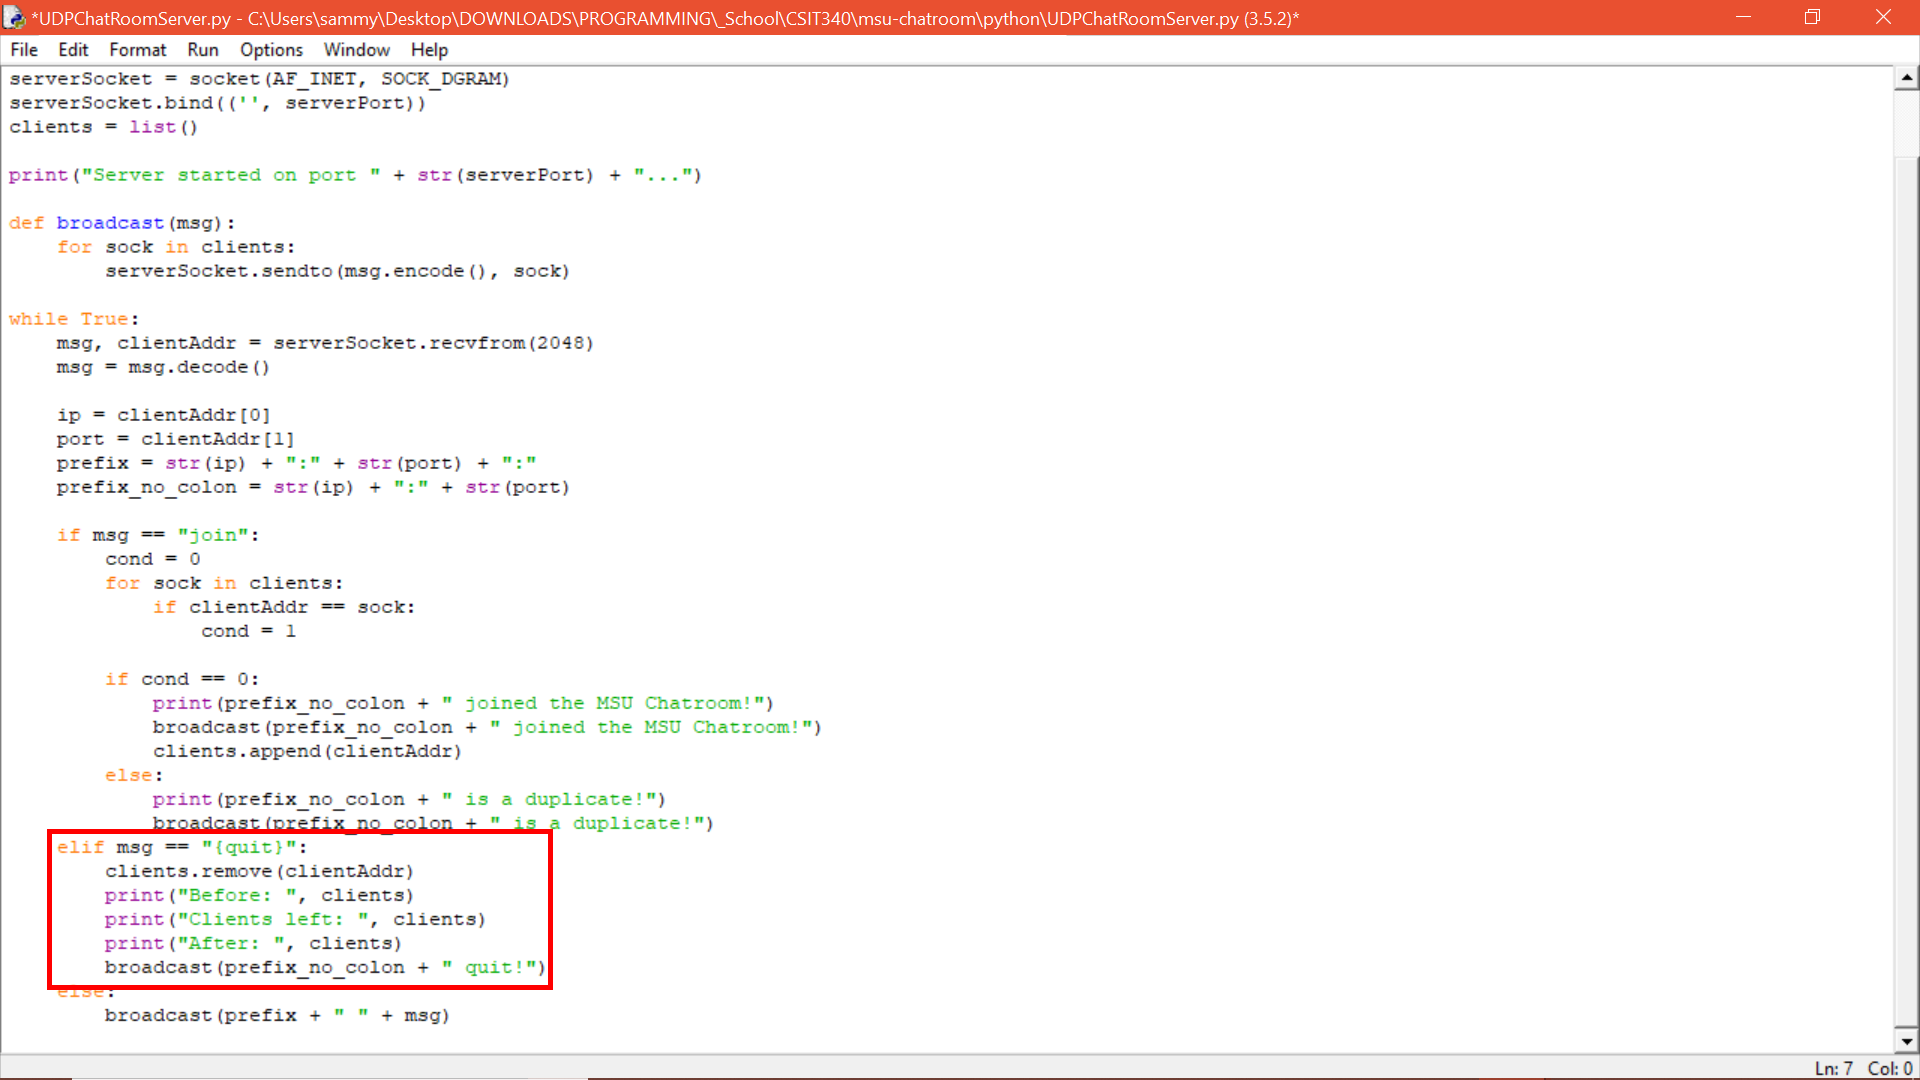
\includegraphics[scale=.25]{test-case-quit.png}\\
\captionof{figure}{Test Case - Quit}
\end{center} \\

\noindent
For the client, there were some requirements that were hard to tell whether they happened correctly or not. We had the most trouble here. Our biggest trouble that we had to figure out was how to make sure the client is receiving and sending at the same time. This was a huge problem that took the most time to figure out. It's simple in theory - create two threads where in one thread it's receiving and another it's sending. But, what the issue was was implementing it. There were several implementations that could of solved this. We were confused on how to do it so we came up with silly implementations like starting up one thread and then going into a while loop that does trigger the thread to start up - that was a huge problem. What we ended up coming up with was to create two unique threads that started and didn't stop execution - and it would stop after both started at the receive.join() method. To ensure that worked, we configured various print statements. Figure 3 shows the implementation. \\

\begin{center}
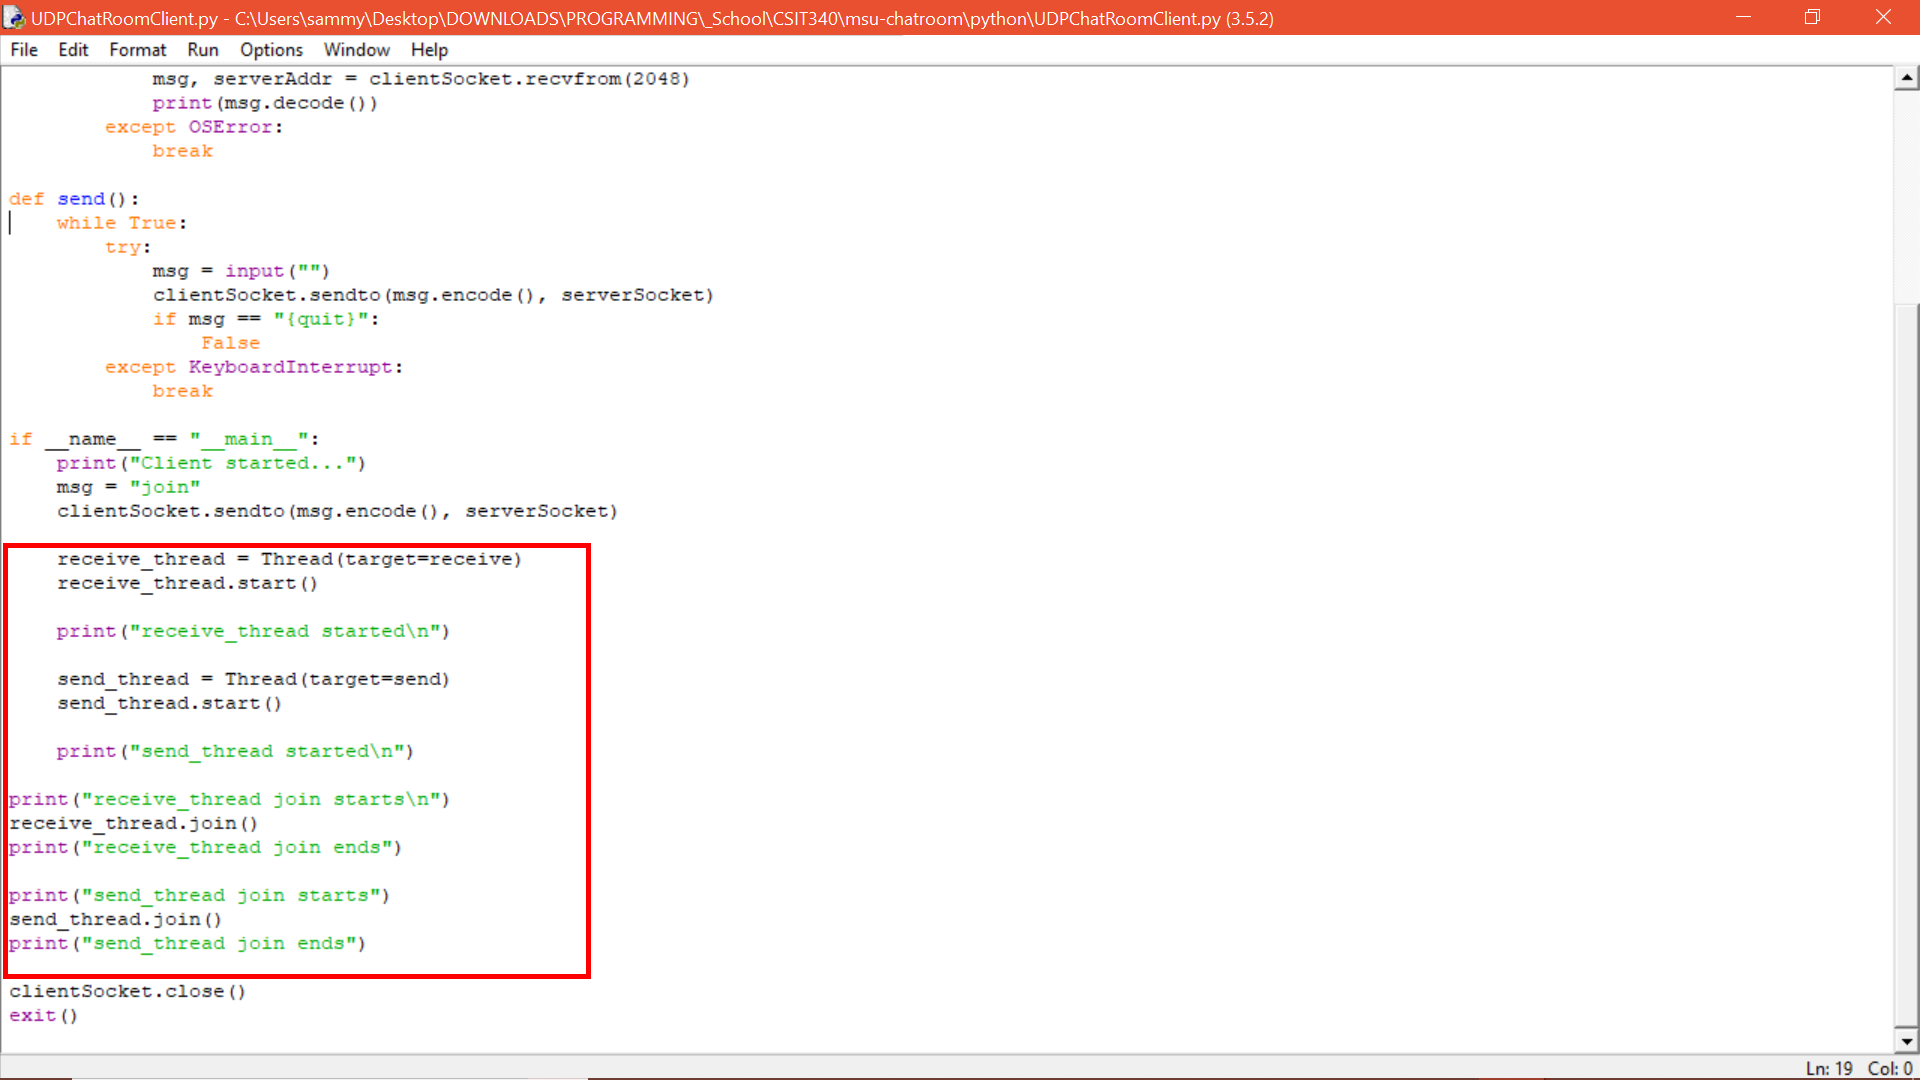
\includegraphics[scale=.25]{test-case-threads.png}\\
\captionof{figure}{Test Case - Threads}
\end{center} \\

\noindent
To ensure that our chat room application works, we created three clients. The server would start up. Then, the first client would join and send several messages to verify it works. The second client would join, which is when we would send messages back and forth between the first and second client to ensure that they work. And then finally, we would have a third client join, where all three of them would be sending messages back and forth to one another. After sending several messages, we would have the second client quit the application. We would verify the first and third client would receive the message that they quit, where then we would send messages back and forth to them again to ensure it still works. We would then quit the third client. We would then verify that the first client received the message that it quit. And then we would quit the first client. Figure 4, 5, 6 and 7 shows that test case.

\begin{center}
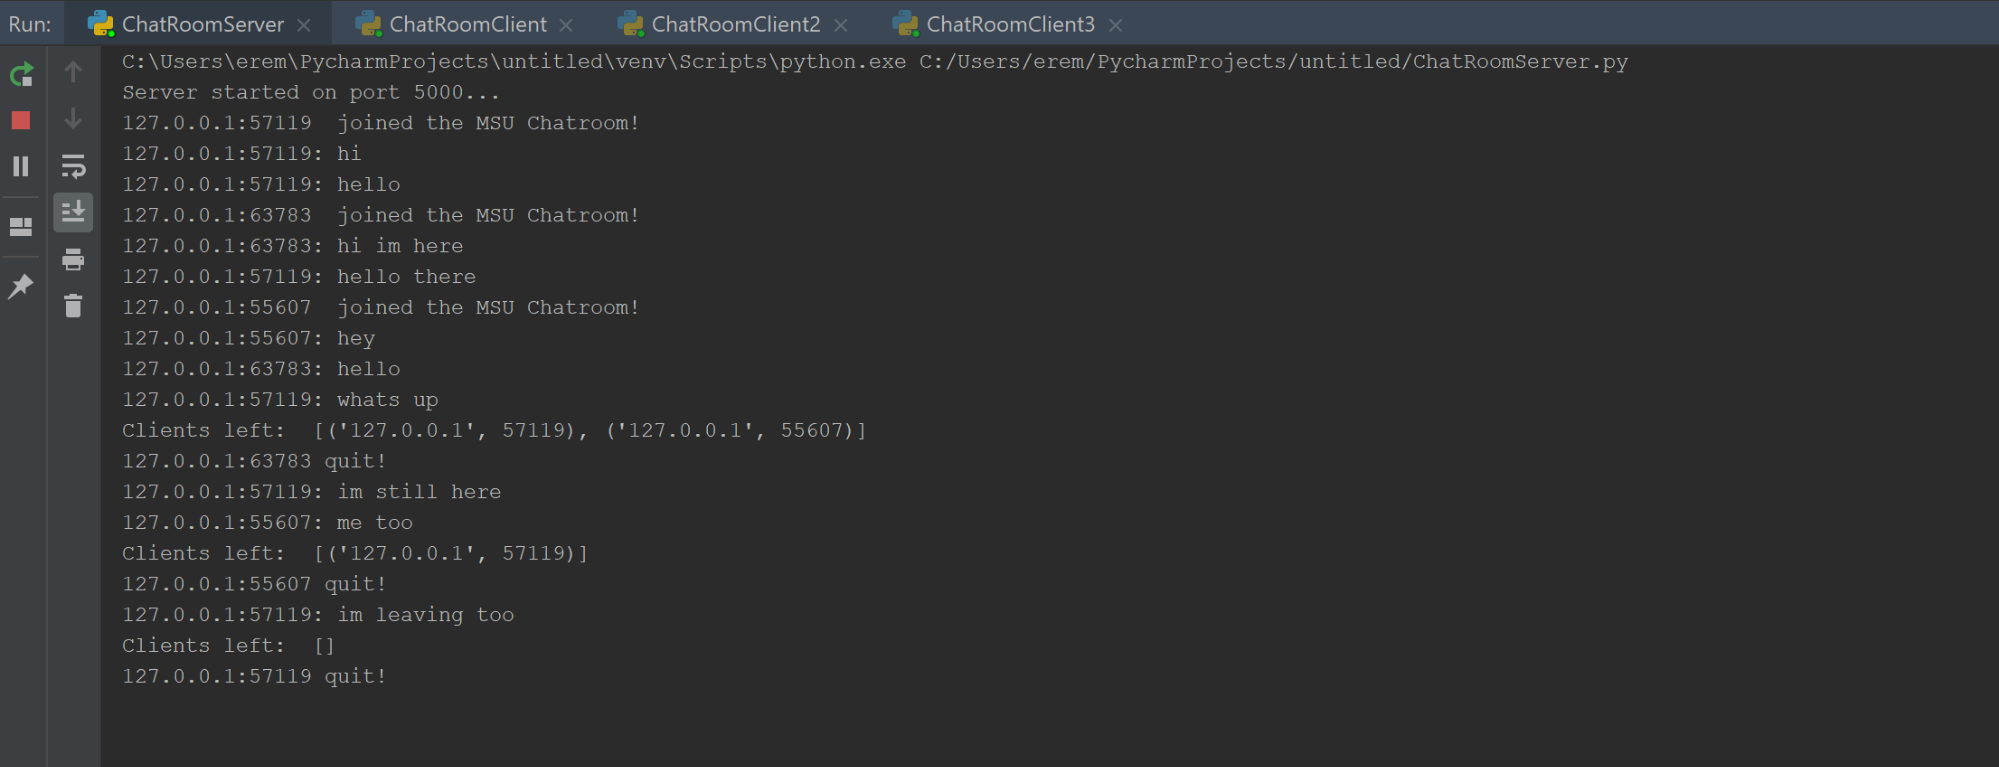
\includegraphics[scale=.2]{chatroom-app-00.png}\\
\captionof{figure}{Test Case - Server}
\end{center} \\

\begin{center}
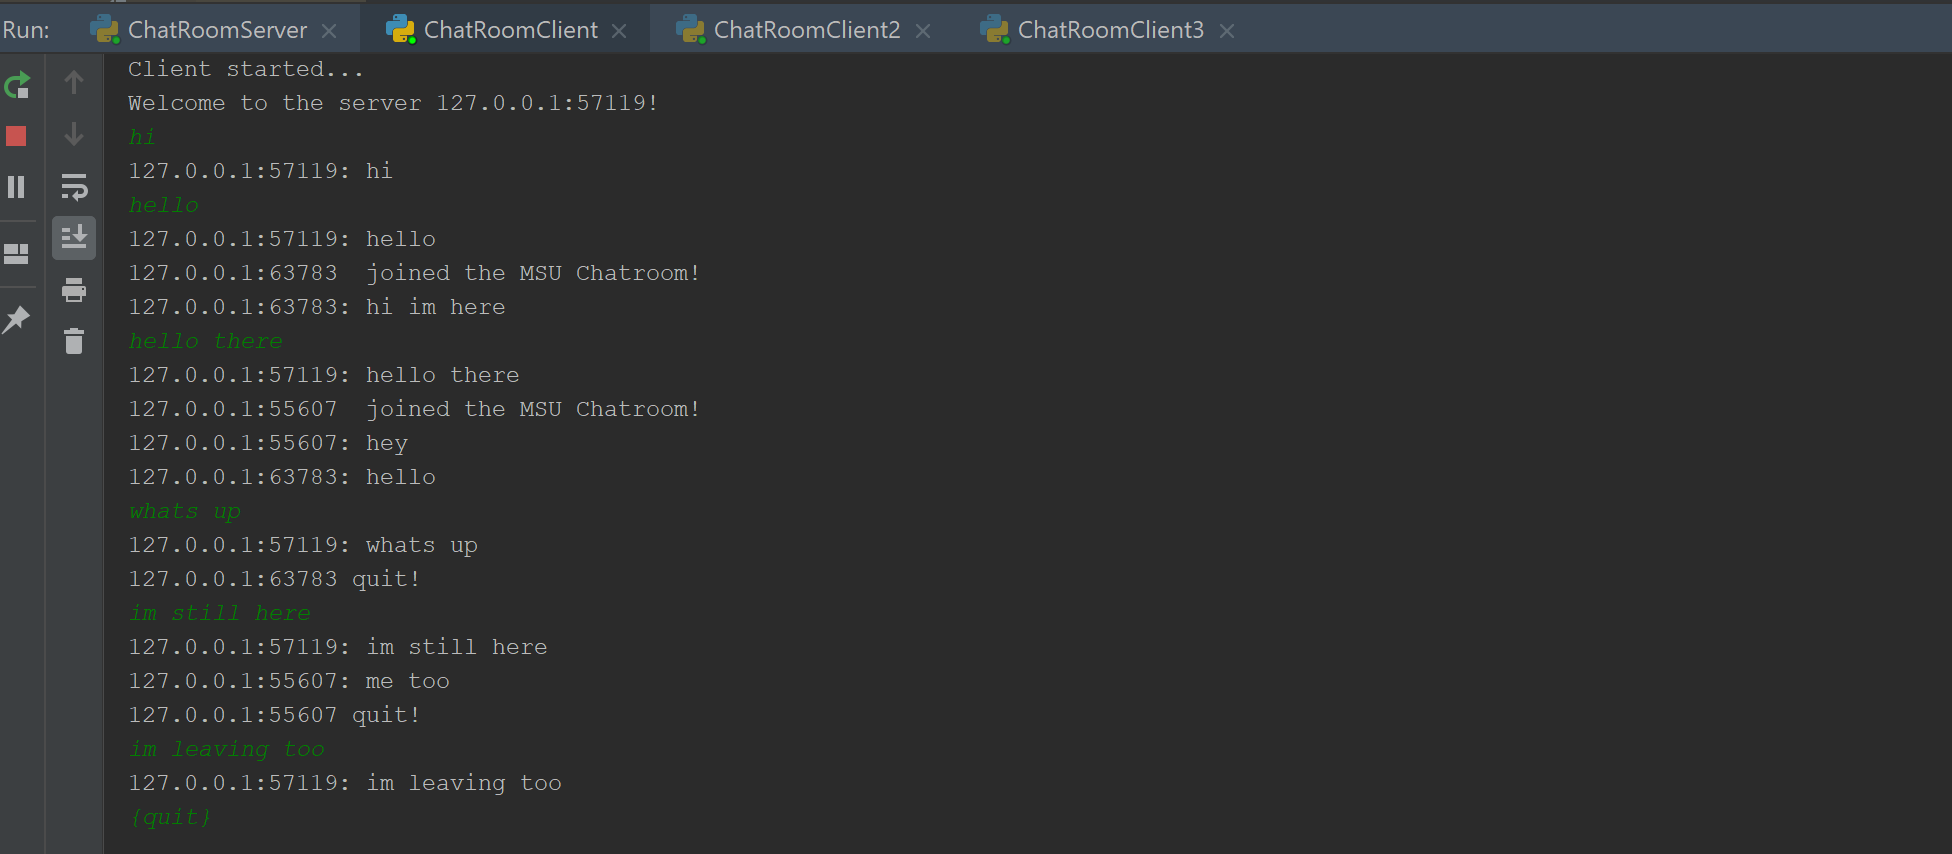
\includegraphics[scale=.2]{chatroom-app-01.png}\\
\captionof{figure}{Test Case - Client 1}
\end{center} \\

\begin{center}
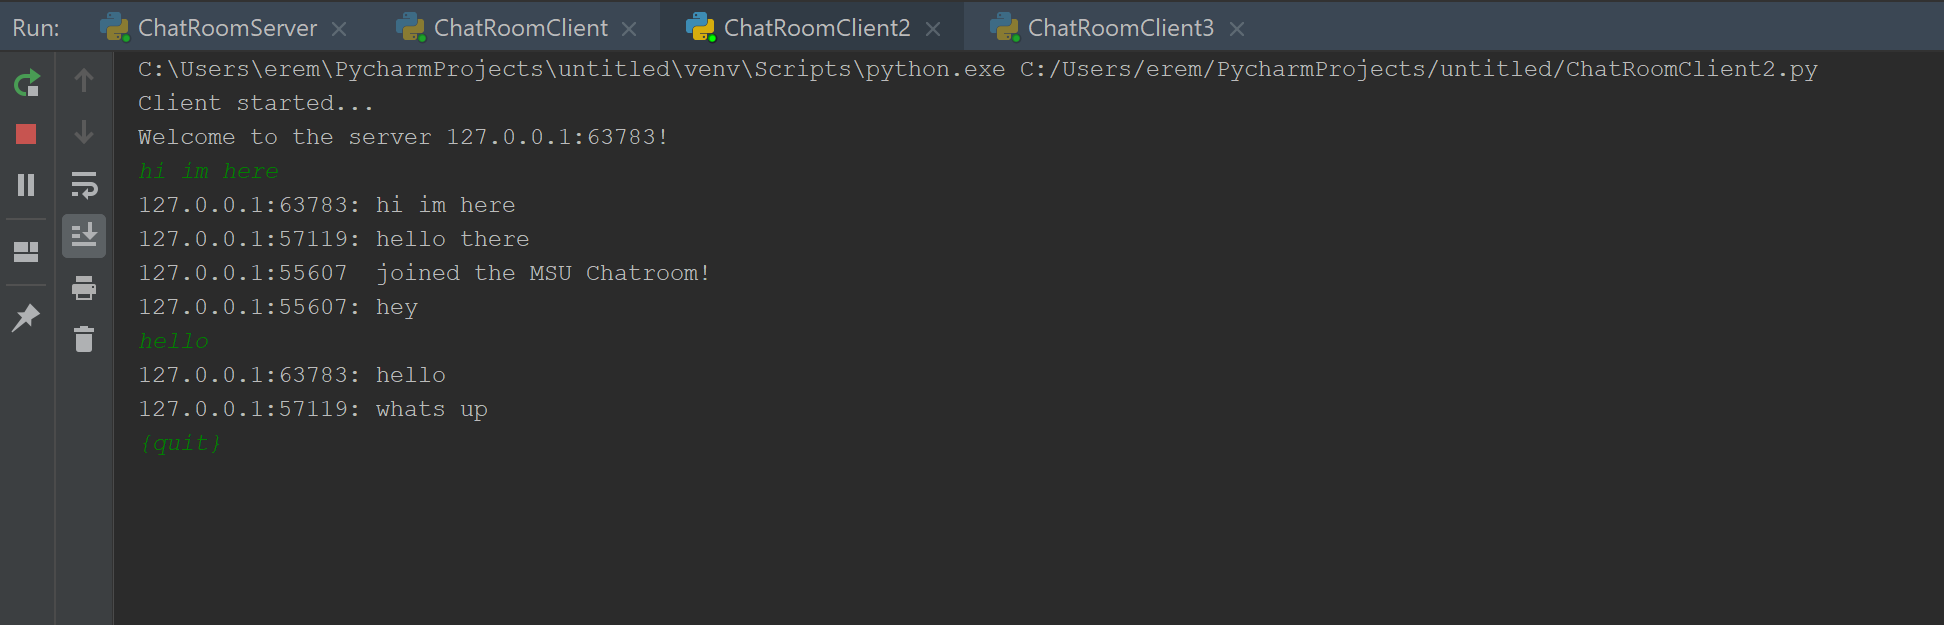
\includegraphics[scale=.2]{chatroom-app-02.png}\\
\captionof{figure}{Test Case - Client 2}
\end{center} \\

\begin{center}
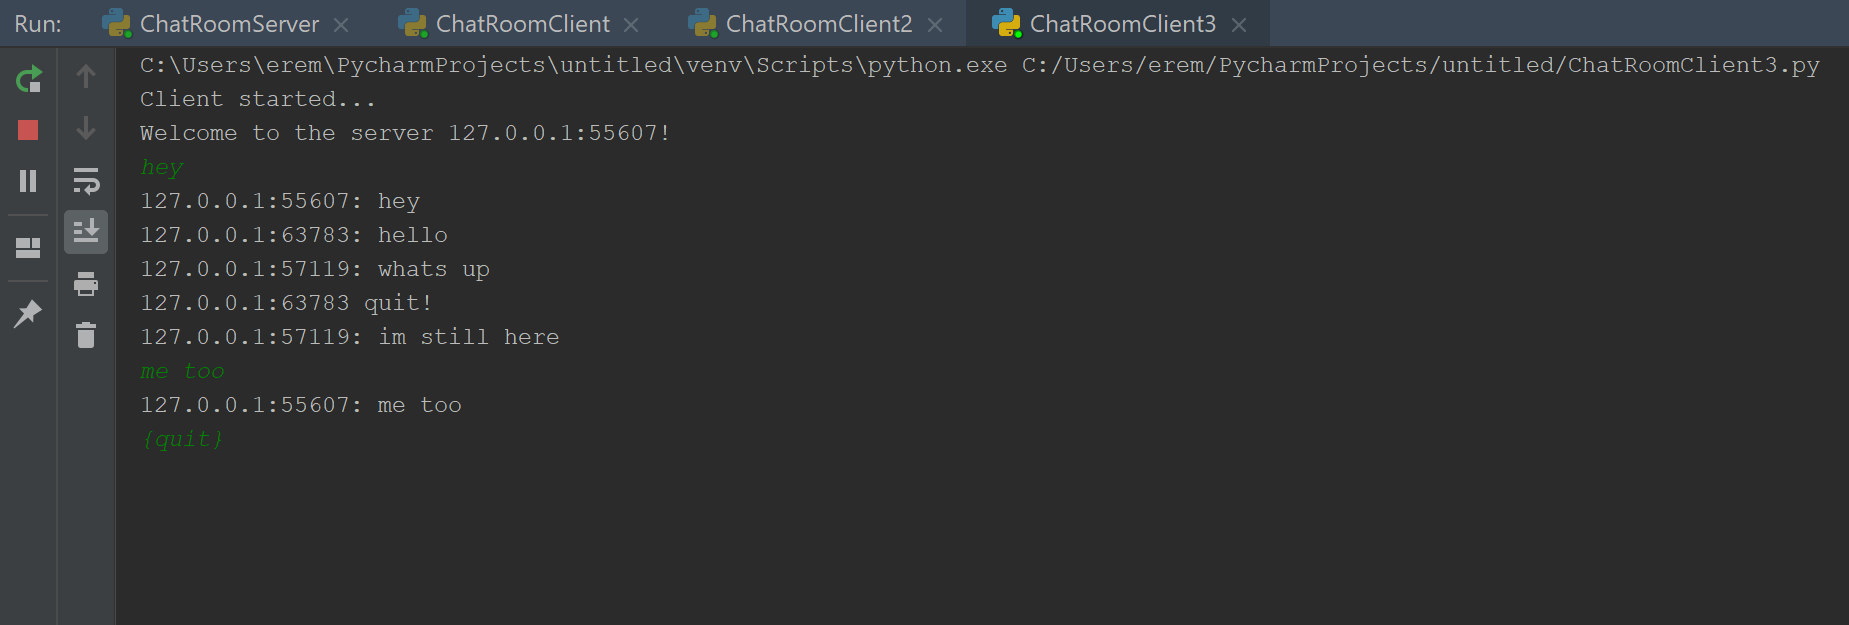
\includegraphics[scale=.2]{chatroom-app-03.png}\\
\captionof{figure}{Test Case - Client 3}
\end{center}

\section{Conclusion}
Each basic requirement has been met, such as supporting multiple clients at the same time, receiving and sending messages at any time, allowing clients to quit the function with ease, etc. However, personal requirements that had been set were not reached due to a setback. Since we initially designed the program around TCP instead of UDP, we had to redesign and implement our entire plan. Originally, we wanted to implement usernames, a GUI, time-stamps, and other things, but since we had a small mixup we did not have the time to do so. That being said, once we had brought the system down to a full design and implementation that we were sure would work; we only had to keep testing and fine-tuning the system. We had meetings where we would discuss how we could think our design was flawed, and how the errors could be occurring. \\

\noindent
Figuring out how errors happened and the way to fix them was only a matter of time since the system itself was not incredibly complex. The project itself, for this reason, was not difficult in terms of understanding and application. However, the troubleshooting itself did take time and several meetings for us to finally burn through. That being said, design and implementation was more difficult while troubleshooting took more time. Overall, the project taught communication, patience, and better application of UDP socket connections.

\end{document}